\subsection{Running an Caesar Program}
Select your Caesar project in the Package Explorer. Drop-down the "run" icon on the toolbar and click "Run..."\\
Select "Java Application" in the left-hand tab and click "New"
Name this configuration "HelloWorld" and then click "Search" to find the main class. Select "HelloWorld".\\\\
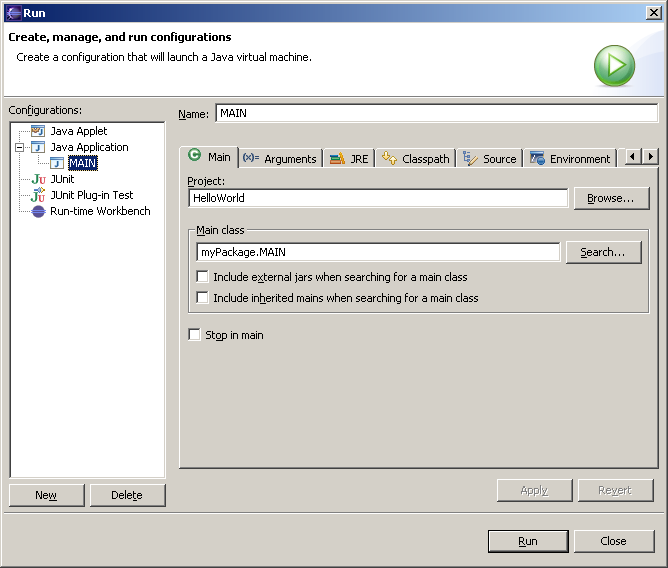
\includegraphics[width=0.80\textwidth]{images/run.png}\\

Click "Apply" and then "Run".\\
You should see the output of the HelloWorld class and the World aspect in the console.\\\\
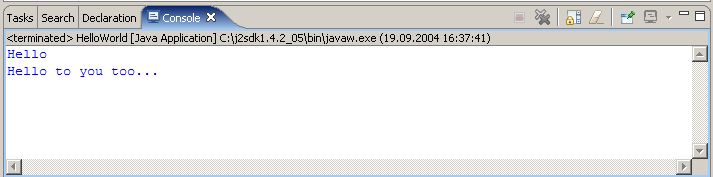
\includegraphics[width=0.80\textwidth]{images/console.png}\\


To run this configuration again, just click on the "run" icon on the toolbar.
